\documentclass[compress,12pt,xcolor={dvipsnames}]{beamer}

\usepackage{pifont}
\usepackage{enumitem}
\usepackage[T1]{fontenc}
\usepackage[utf8]{inputenc}
\usepackage{listings}
\usepackage{amssymb}
\usepackage{color}
\usepackage{scalerel,xparse}

\newlist{checklist}{itemize}{2}
\setlist[checklist]{label=$\square$}
\newcommand{\cmark}{\ding{51}}%
\newcommand{\xmark}{\ding{55}}%
\newcommand{\done}{\rlap{$\square$}{\raisebox{2pt}{\large\hspace{1pt}\cmark}}%
\hspace{-2.5pt}}
\newcommand{\wontfix}{\rlap{$\square$}{\large\hspace{1pt}\xmark}}

% \addtobeamertemplate{note page}{}{\thispdfpagelabel{notes:\insertframenumber}}
% \setbeameroption{show notes on second screen}

\graphicspath{ {./assets/} }
\NewDocumentCommand\emojicamel{}{
    \scalerel*{
        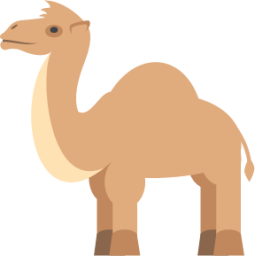
\includegraphics{camel_emoji.png}
    }{X}
}

\usetheme{Arguelles}

\title{Software correctness}
\subtitle{We can and know how to do better}
\event{}
\date{}
\author{Marcin Wojnarowski}
\institute{Fluttercon 2024}
% TODO: Does not work
% \email{name@domain.com}
\homepage{shilangyu.dev}
\github{shilangyu}

\definecolor{keywordcolor}{rgb}{0.7, 0.1, 0.1}   % red
\definecolor{tacticcolor}{rgb}{0.0, 0.1, 0.6}    % blue
\definecolor{commentcolor}{rgb}{0.4, 0.4, 0.4}   % grey
\definecolor{symbolcolor}{rgb}{0.0, 0.1, 0.6}    % blue
\definecolor{sortcolor}{rgb}{0.1, 0.5, 0.1}      % green
\definecolor{attributecolor}{rgb}{0.7, 0.1, 0.1} % red

\def\lstlanguagefiles{lstlean.tex}
\lstdefinelanguage{Oop}{
  keywords={func, class, extends, var, throw, if, self, return, override, constructor},
  ndkeywords={true, false},
  sensitive=false,
  comment=[l]{\#},
}

\lstdefinelanguage{typescript}{
  keywords={type, function, if, else, typeof, satisfies},
  ndkeywords={true, false},
  sensitive=false,
  comment=[l]{\#},
}

\lstdefinelanguage{Cpp}{
  keywords={\#include},
  ndkeywords={int},
  sensitive=false,
  comment=[l]{//},
}

\lstdefinelanguage{TypeState}{
  keywords={func, class, typestate, transition_to, when, with},
  emph={int, string},
  sensitive=false,
  comment=[l]{\#},
}

\lstdefinelanguage{Koka}{
  keywords={effect, ctl, fun, val, var, return, if, handler, then},
  emph={bool, False, True, println},
  sensitive=false,
  comment=[l]{\#},
}

\lstdefinelanguage{Dart}{
  keywords={class, if, else},
  emph={int, string, void, print},
  sensitive=false,
  comment=[l]{//},
}

\lstdefinelanguage{Kotlin}{
  comment=[l]{//},
  emph={filter, first, firstOrNull, forEach, lazy, map, mapNotNull, println},
  keywords={!in, !is, abstract, actual, annotation, as, as?, break, by, catch, class, companion, const, constructor, continue, crossinline, data, delegate, do, dynamic, else, enum, expect, external, false, field, file, final, finally, for, fun, get, if, import, in, infix, init, inline, inner, interface, internal, is, lateinit, noinline, null, object, open, operator, out, override, package, param, private, property, protected, public, receiveris, reified, return, return@, sealed, set, setparam, super, suspend, tailrec, this, throw, true, try, typealias, typeof, val, var, vararg, when, where, while},
  morecomment=[s]{/*}{*/},
  morestring=[b]",
  morestring=[s]{"""*}{*"""},
  ndkeywords={@Deprecated, @JvmField, @JvmName, @JvmOverloads, @JvmStatic, @JvmSynthetic, Array, Byte, Double, Float, Int, Integer, Iterable, Long, Runnable, Short, String, Any, Unit, Nothing},
}

\lstdefinelanguage{Rust}{%
sensitive%
, morecomment=[l]{//}%
, morecomment=[s]{/*}{*/}%
, moredelim=[s][{\itshape\color[rgb]{0,0,0.75}}]{\#[}{]}%
, morestring=[b]{"}%
, alsodigit={}%
, alsoother={}%
, alsoletter={!}%
%
%
% [1] reserve keywords
% [2] traits
% [3] primitive types
% [4] type and value constructors
% [5] identifier
%
, morekeywords={break, continue, else, for, if, in, loop, match, return, while}  % control flow keywords
, morekeywords={as, const, let, move, mut, ref, static}  % in the context of variables
, morekeywords={dyn, enum, fn, impl, Self, self, struct, trait, type, union, use, where}  % in the context of declarations
, morekeywords={crate, extern, mod, pub, super}  % in the context of modularisation
, morekeywords={unsafe}  % markers
, morekeywords={abstract, alignof, become, box, do, final, macro, offsetof, override, priv, proc, pure, sizeof, typeof, unsized, virtual, yield}  % reserved identifiers
%
% grep 'pub trait [A-Za-z][A-Za-z0-9]*' -r . | sed 's/^.*pub trait \([A-Za-z][A-Za-z0-9]*\).*/\1/g' | sort -u | tr '\n' ',' | sed 's/^\(.*\),$/{\1}\n/g' | sed 's/,/, /g'
, morekeywords=[2]{Add, AddAssign, Any, AsciiExt, AsInner, AsInnerMut, AsMut, AsRawFd, AsRawHandle, AsRawSocket, AsRef, Binary, BitAnd, BitAndAssign, Bitor, BitOr, BitOrAssign, BitXor, BitXorAssign, Borrow, BorrowMut, Boxed, BoxPlace, BufRead, BuildHasher, CastInto, CharExt, Clone, CoerceUnsized, CommandExt, Copy, Debug, DecodableFloat, Default, Deref, DerefMut, DirBuilderExt, DirEntryExt, Display, Div, DivAssign, DoubleEndedIterator, DoubleEndedSearcher, Drop, EnvKey, Eq, Error, ExactSizeIterator, ExitStatusExt, Extend, FileExt, FileTypeExt, Float, Fn, FnBox, FnMut, FnOnce, Freeze, From, FromInner, FromIterator, FromRawFd, FromRawHandle, FromRawSocket, FromStr, FullOps, FusedIterator, Generator, Hash, Hasher, Index, IndexMut, InPlace, Int, Into, IntoCow, IntoInner, IntoIterator, IntoRawFd, IntoRawHandle, IntoRawSocket, IsMinusOne, IsZero, Iterator, JoinHandleExt, LargeInt, LowerExp, LowerHex, MetadataExt, Mul, MulAssign, Neg, Not, Octal, OpenOptionsExt, Ord, OsStrExt, OsStringExt, Packet, PartialEq, PartialOrd, Pattern, PermissionsExt, Place, Placer, Pointer, Product, Put, RangeArgument, RawFloat, Read, Rem, RemAssign, Seek, Shl, ShlAssign, Shr, ShrAssign, Sized, SliceConcatExt, SliceExt, SliceIndex, Stats, Step, StrExt, Sub, SubAssign, Sum, Sync, TDynBenchFn, Terminal, Termination, ToOwned, ToSocketAddrs, ToString, Try, TryFrom, TryInto, UnicodeStr, Unsize, UpperExp, UpperHex, WideInt, Write}
, morekeywords=[2]{Send}  % additional traits
%
, morekeywords=[3]{bool, char, f32, f64, i8, i16, i32, i64, isize, str, u8, u16, u32, u64, unit, usize, i128, u128}  % primitive types
%
, morekeywords=[4]{Err, false, None, Ok, Some, true}  % prelude value constructors
% grep 'pub \(type\|struct\|enum\) [A-Za-z][A-Za-z0-9]*' -r . | sed 's/^.*pub \(type\|struct\|enum\) \([A-Za-z][A-Za-z0-9]*\).*/\2/g' | sort -u | tr '\n' ',' | sed 's/^\(.*\),$/{\1}\n/g' | sed 's/,/, /g'    
, morekeywords=[3]{AccessError, Adddf3, AddI128, AddoI128, AddoU128, ADDRESS, ADDRESS64, addrinfo, ADDRINFOA, AddrParseError, Addsf3, AddU128, advice, aiocb, Alignment, AllocErr, AnonPipe, Answer, Arc, Args, ArgsInnerDebug, ArgsOs, Argument, Arguments, ArgumentV1, Ashldi3, Ashlti3, Ashrdi3, Ashrti3, AssertParamIsClone, AssertParamIsCopy, AssertParamIsEq, AssertUnwindSafe, AtomicBool, AtomicPtr, Attr, auxtype, auxv, BackPlace, BacktraceContext, Barrier, BarrierWaitResult, Bencher, BenchMode, BenchSamples, BinaryHeap, BinaryHeapPlace, blkcnt, blkcnt64, blksize, BOOL, boolean, BOOLEAN, BoolTrie, BorrowError, BorrowMutError, Bound, Box, bpf, BTreeMap, BTreeSet, Bucket, BucketState, Buf, BufReader, BufWriter, Builder, BuildHasherDefault, BY, BYTE, Bytes, CannotReallocInPlace, cc, Cell, Chain, CHAR, CharIndices, CharPredicateSearcher, Chars, CharSearcher, CharsError, CharSliceSearcher, CharTryFromError, Child, ChildPipes, ChildStderr, ChildStdin, ChildStdio, ChildStdout, Chunks, ChunksMut, ciovec, clock, clockid, Cloned, cmsgcred, cmsghdr, CodePoint, Color, ColorConfig, Command, CommandEnv, Component, Components, CONDITION, condvar, Condvar, CONSOLE, CONTEXT, Count, Cow, cpu, CRITICAL, CStr, CString, CStringArray, Cursor, Cycle, CycleIter, daddr, DebugList, DebugMap, DebugSet, DebugStruct, DebugTuple, Decimal, Decoded, DecodeUtf16, DecodeUtf16Error, DecodeUtf8, DefaultEnvKey, DefaultHasher, dev, device, Difference, Digit32, DIR, DirBuilder, dircookie, dirent, dirent64, DirEntry, Discriminant, DISPATCHER, Display, Divdf3, Divdi3, Divmoddi4, Divmodsi4, Divsf3, Divsi3, Divti3, dl, Dl, Dlmalloc, Dns, DnsAnswer, DnsQuery, dqblk, Drain, DrainFilter, Dtor, Duration, DwarfReader, DWORD, DWORDLONG, DynamicLibrary, Edge, EHAction, EHContext, Elf32, Elf64, Empty, EmptyBucket, EncodeUtf16, EncodeWide, Entry, EntryPlace, Enumerate, Env, epoll, errno, Error, ErrorKind, EscapeDebug, EscapeDefault, EscapeUnicode, event, Event, eventrwflags, eventtype, ExactChunks, ExactChunksMut, EXCEPTION, Excess, ExchangeHeapSingleton, exit, exitcode, ExitStatus, Failure, fd, fdflags, fdsflags, fdstat, ff, fflags, File, FILE, FileAttr, filedelta, FileDesc, FilePermissions, filesize, filestat, FILETIME, filetype, FileType, Filter, FilterMap, Fixdfdi, Fixdfsi, Fixdfti, Fixsfdi, Fixsfsi, Fixsfti, Fixunsdfdi, Fixunsdfsi, Fixunsdfti, Fixunssfdi, Fixunssfsi, Fixunssfti, Flag, FlatMap, Floatdidf, FLOATING, Floatsidf, Floatsisf, Floattidf, Floattisf, Floatundidf, Floatunsidf, Floatunsisf, Floatuntidf, Floatuntisf, flock, ForceResult, FormatSpec, Formatted, Formatter, Fp, FpCategory, fpos, fpos64, fpreg, fpregset, FPUControlWord, Frame, FromBytesWithNulError, FromUtf16Error, FromUtf8Error, FrontPlace, fsblkcnt, fsfilcnt, fsflags, fsid, fstore, fsword, FullBucket, FullBucketMut, FullDecoded, Fuse, GapThenFull, GeneratorState, gid, glob, glob64, GlobalDlmalloc, greg, group, GROUP, Guard, GUID, Handle, HANDLE, Handler, HashMap, HashSet, Heap, HINSTANCE, HMODULE, hostent, HRESULT, id, idtype, if, ifaddrs, IMAGEHLP, Immut, in, in6, Incoming, Infallible, Initializer, ino, ino64, inode, input, InsertResult, Inspect, Instant, int16, int32, int64, int8, integer, IntermediateBox, Internal, Intersection, intmax, IntoInnerError, IntoIter, IntoStringError, intptr, InvalidSequence, iovec, ip, IpAddr, ipc, Ipv4Addr, ipv6, Ipv6Addr, Ipv6MulticastScope, Iter, IterMut, itimerspec, itimerval, jail, JoinHandle, JoinPathsError, KDHELP64, kevent, kevent64, key, Key, Keys, KV, l4, LARGE, lastlog, launchpad, Layout, Lazy, lconv, Leaf, LeafOrInternal, Lines, LinesAny, LineWriter, linger, linkcount, LinkedList, load, locale, LocalKey, LocalKeyState, Location, lock, LockResult, loff, LONG, lookup, lookupflags, LookupHost, LPBOOL, LPBY, LPBYTE, LPCSTR, LPCVOID, LPCWSTR, LPDWORD, LPFILETIME, LPHANDLE, LPOVERLAPPED, LPPROCESS, LPPROGRESS, LPSECURITY, LPSTARTUPINFO, LPSTR, LPVOID, LPWCH, LPWIN32, LPWSADATA, LPWSAPROTOCOL, LPWSTR, Lshrdi3, Lshrti3, lwpid, M128A, mach, major, Map, mcontext, Metadata, Metric, MetricMap, mflags, minor, mmsghdr, Moddi3, mode, Modsi3, Modti3, MonitorMsg, MOUNT, mprot, mq, mqd, msflags, msghdr, msginfo, msglen, msgqnum, msqid, Muldf3, Mulodi4, Mulosi4, Muloti4, Mulsf3, Multi3, Mut, Mutex, MutexGuard, MyCollection, n16, NamePadding, NativeLibBoilerplate, nfds, nl, nlink, NodeRef, NoneError, NonNull, NonZero, nthreads, NulError, OccupiedEntry, off, off64, oflags, Once, OnceState, OpenOptions, Option, Options, OptRes, Ordering, OsStr, OsString, Output, OVERLAPPED, Owned, Packet, PanicInfo, Param, ParseBoolError, ParseCharError, ParseError, ParseFloatError, ParseIntError, ParseResult, Part, passwd, Path, PathBuf, PCONDITION, PCONSOLE, Peekable, PeekMut, Permissions, PhantomData, pid, Pipes, PlaceBack, PlaceFront, PLARGE, PoisonError, pollfd, PopResult, port, Position, Powidf2, Powisf2, Prefix, PrefixComponent, PrintFormat, proc, Process, PROCESS, processentry, protoent, PSRWLOCK, pthread, ptr, ptrdiff, PVECTORED, Queue, radvisory, RandomState, Range, RangeFrom, RangeFull, RangeInclusive, RangeMut, RangeTo, RangeToInclusive, RawBucket, RawFd, RawHandle, RawPthread, RawSocket, RawTable, RawVec, Rc, ReadDir, Receiver, recv, RecvError, RecvTimeoutError, ReentrantMutex, ReentrantMutexGuard, Ref, RefCell, RefMut, REPARSE, Repeat, Result, Rev, Reverse, riflags, rights, rlim, rlim64, rlimit, rlimit64, roflags, Root, RSplit, RSplitMut, RSplitN, RSplitNMut, RUNTIME, rusage, RwLock, RWLock, RwLockReadGuard, RwLockWriteGuard, sa, SafeHash, Scan, sched, scope, sdflags, SearchResult, SearchStep, SECURITY, SeekFrom, segment, Select, SelectionResult, sem, sembuf, send, Sender, SendError, servent, sf, Shared, shmatt, shmid, ShortReader, ShouldPanic, Shutdown, siflags, sigaction, SigAction, sigevent, sighandler, siginfo, Sign, signal, signalfd, SignalToken, sigset, sigval, Sink, SipHasher, SipHasher13, SipHasher24, size, SIZE, Skip, SkipWhile, Slice, SmallBoolTrie, sockaddr, SOCKADDR, sockcred, Socket, SOCKET, SocketAddr, SocketAddrV4, SocketAddrV6, socklen, speed, Splice, Split, SplitMut, SplitN, SplitNMut, SplitPaths, SplitWhitespace, spwd, SRWLOCK, ssize, stack, STACKFRAME64, StartResult, STARTUPINFO, stat, Stat, stat64, statfs, statfs64, StaticKey, statvfs, StatVfs, statvfs64, Stderr, StderrLock, StderrTerminal, Stdin, StdinLock, Stdio, StdioPipes, Stdout, StdoutLock, StdoutTerminal, StepBy, String, StripPrefixError, StrSearcher, subclockflags, Subdf3, SubI128, SuboI128, SuboU128, subrwflags, subscription, Subsf3, SubU128, Summary, suseconds, SYMBOL, SYMBOLIC, SymmetricDifference, SyncSender, sysinfo, System, SystemTime, SystemTimeError, Take, TakeWhile, tcb, tcflag, TcpListener, TcpStream, TempDir, TermInfo, TerminfoTerminal, termios, termios2, TestDesc, TestDescAndFn, TestEvent, TestFn, TestName, TestOpts, TestResult, Thread, threadattr, threadentry, ThreadId, tid, time, time64, timespec, TimeSpec, timestamp, timeval, timeval32, timezone, tm, tms, ToLowercase, ToUppercase, TraitObject, TryFromIntError, TryFromSliceError, TryIter, TryLockError, TryLockResult, TryRecvError, TrySendError, TypeId, U64x2, ucontext, ucred, Udivdi3, Udivmoddi4, Udivmodsi4, Udivmodti4, Udivsi3, Udivti3, UdpSocket, uid, UINT, uint16, uint32, uint64, uint8, uintmax, uintptr, ulflags, ULONG, ULONGLONG, Umoddi3, Umodsi3, Umodti3, UnicodeVersion, Union, Unique, UnixDatagram, UnixListener, UnixStream, Unpacked, UnsafeCell, UNWIND, UpgradeResult, useconds, user, userdata, USHORT, Utf16Encoder, Utf8Error, Utf8Lossy, Utf8LossyChunk, Utf8LossyChunksIter, utimbuf, utmp, utmpx, utsname, uuid, VacantEntry, Values, ValuesMut, VarError, Variables, Vars, VarsOs, Vec, VecDeque, vm, Void, WaitTimeoutResult, WaitToken, wchar, WCHAR, Weak, whence, WIN32, WinConsole, Windows, WindowsEnvKey, winsize, WORD, Wrapping, wrlen, WSADATA, WSAPROTOCOL, WSAPROTOCOLCHAIN, Wtf8, Wtf8Buf, Wtf8CodePoints, xsw, xucred, Zip, zx}
%
, morekeywords=[5]{assert!, assert_eq!, assert_ne!, cfg!, column!, compile_error!, concat!, concat_idents!, debug_assert!, debug_assert_eq!, debug_assert_ne!, env!, eprint!, eprintln!, file!, format!, format_args!, include!, include_bytes!, include_str!, line!, module_path!, option_env!, panic!, print!, println!, select!, stringify!, thread_local!, try!, unimplemented!, unreachable!, vec!, write!, writeln!}  % prelude macros
}%

\lstdefinelanguage{CSharp}{
  morecomment=[l]{//}, %use comment-line-style!
  morecomment=[l]{\#}, %use comment-line-style!
  morecomment=[s]{/*}{*/}, %for multiline comments
  morekeywords={ abstract, event, new, struct,
      as, explicit, null, switch,
      base, extern, object, this,
      bool, false, operator, throw,
      break, finally, out, true,
      byte, fixed, override, try,
      case, float, params, typeof,
      catch, for, private, uint,
      char, foreach, protected, ulong,
      checked, goto, public, unchecked,
      class, if, readonly, unsafe,
      const, implicit, ref, ushort,
      continue, in, return, using,
      decimal, int, sbyte, virtual,
      default, interface, sealed, volatile,
      delegate, internal, short, void,
      do, is, sizeof, while,
      double, lock, stackalloc,
      else, long, static,
      enum, namespace, string, var},
  morestring=[b]",
}

\lstset{
  breaklines=true,
  numbers=left,
  numberstyle=\scriptsize\color{black},
  escapechar=@,
  commentstyle={\color{gray}\ttfamily},
  emphstyle={\color{OrangeRed}},
  identifierstyle=\color{black}\ttfamily,
  keywordstyle={\color{NavyBlue}\bfseries},
  sensitive=true,
  stringstyle={\color{ForestGreen}\ttfamily},
  basicstyle=\linespread{0.5}\tt\footnotesize
}


\begin{document}

\frame[plain]{\titlepage

    \note[item]{The goal of the presentation is to expose you to topics that appear casually in academia, but are not often discussed in the industry.}
}


\begin{frame}
    \frametitle{Who is me?}
    \framesubtitle{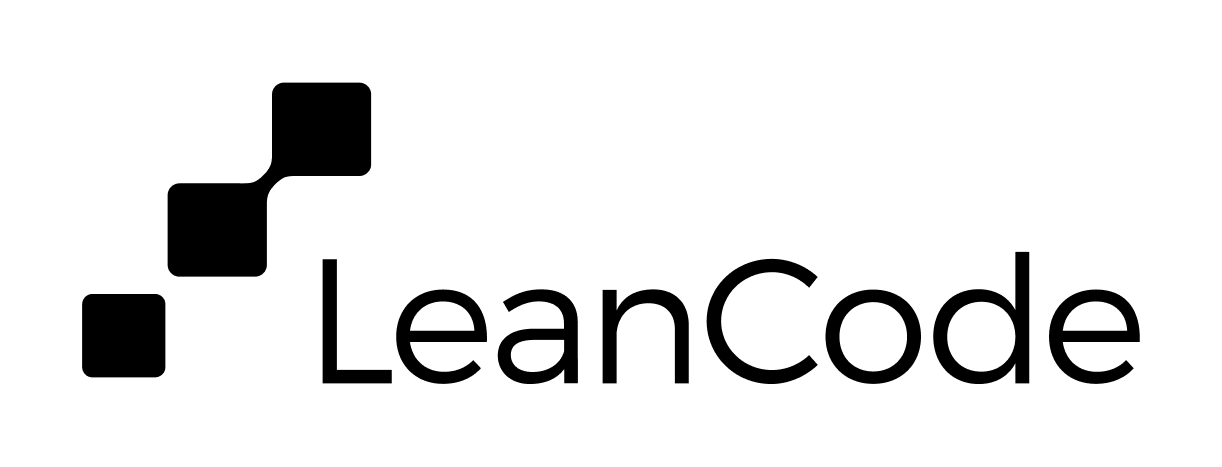
\includegraphics[width=0.35\textwidth]{leancode_logo.png}}

    \begin{enumerate}
        \item Senior developer at LeanCode (now technically an intern)
        \item Connected to the academic and industry worlds
        \item Interested in programming language theory
    \end{enumerate}
\end{frame}


\begin{frame}
    \begin{block}{Disclaimer 1}
        Many simplifications have been done to make this presentation digestible.
    \end{block}
    \begin{alertblock}{Disclaimer 2}
        Presentation contains potentially controversial opinions. Those will be annotated with a red label like this disclaimer.
    \end{alertblock}
    \begin{block}{Disclaimer 3}
        Interrupt me if something isn't clear. Unless it is to fight a controversial opinion that was presented, leave this for after the presentation.
    \end{block}
    \note[item]{Disclaimer 3: what a convenient way for me to avoid public humiliation.}
    \note[item]{Many languages will appear, don't get too comfortable.}
\end{frame}


\begin{frame}[standout]
    \centering\large
    I \textbf{\itshape don't} like to write tests\note[itemize]{
        \item I feel like people are ashamed to admit that
        \item That isn't to say I don't think they are valuable,
        \item but it mostly feels like only a best-effort approach that has zero guarantees: functions can be written to only pass tests while not doing anything useful. A fixed set of points can always be interpolated by a function.
        \item People have devoted a lot of time trying to define what a valuable test is. Very engineering approach, I don't like it.
    }
\end{frame}

\section{Programming languages}
\begin{frame}
    \frametitle{\\Why do programming languages exist?}
    \framesubtitle{\\Why are new ones being created daily?}\note[item]{Granted, it is not as often as js UI frameworks}

    \begin{enumerate}
        \item To simplify how we express ideas in code \note[item]{Example: In Zig allocation is not implicit, metaprogramming and runtime is merged.}\pause
        \item \textbf{To give correctness guarantees}\note[itemize]{
        \item I love new programming languages, but not all of them.
        \item I am NOT on the mojo hype. I dislike Python, mojo doesn't introduce any safety nor usability feature that interest me.
              } \note[item]{CROWD: any ideas for a very fundamental language feature that makes software more correct?}
    \end{enumerate}
\end{frame}

\begin{frame}{Example features}
    \note[item]{Features that exist in mainstream languages}
    \begin{itemize}
        \item Types!
              \only<1>{\begin{alertblock}{Opinion}
                      I don't understand why people unironically write large software in languages without static types \note[item]{Noticed how mainstream interpreted languages are getting types? (Python, Typescript)}
                  \end{alertblock}}\pause
        \item Null safety: \texttt{T?}\quad \texttt{?T}\quad \texttt{T | null} \note[item]{Not always taken seriously: Kotlin, C\#}
        \item Memory safety: memory is always initialized, memory is always valid \note[itemize]{
        \item High level languages usually get memory safety (garbage collection helps alot with reference validity)
        \item Lower level languages give these guarantees by special semantics of the type system (borrow checker in Rust, value semantics in Swift)
              }
    \end{itemize}
\end{frame}

\subsection{Null safety}
\begin{frame}[fragile]{Null "safety"}
    \framesubtitle{Kotlin}
    \centering{
\includegraphics[width=0.65\textwidth]{kotlin_null_safety.png}}
    \begin{lstlisting}[gobble=8,language=Kotlin,basicstyle=\footnotesize]
        class Foo {
            val bar: String = makeBar()
            val qux: String = ""
            fun makeBar(): String = qux
        }
        
        fun main() {
            println(Foo().bar) // -> null
        }
        \end{lstlisting}
\end{frame}

\begin{frame}[fragile]{Nullable references}
    \framesubtitle{C\#}
    \begin{lstlisting}[gobble=8,language=CSharp,basicstyle=\scriptsize]
        var _ = new Foo();
        
        class Bar {
            static public void DontMindMe(Foo f) {
                Console.WriteLine(f.s);
            }
        }
        
        class Foo {
            public String s;
            public Foo() {
                Bar.DontMindMe(this);
                s = "hello";
            }
        }
        \end{lstlisting}
    \only<1>{\centering{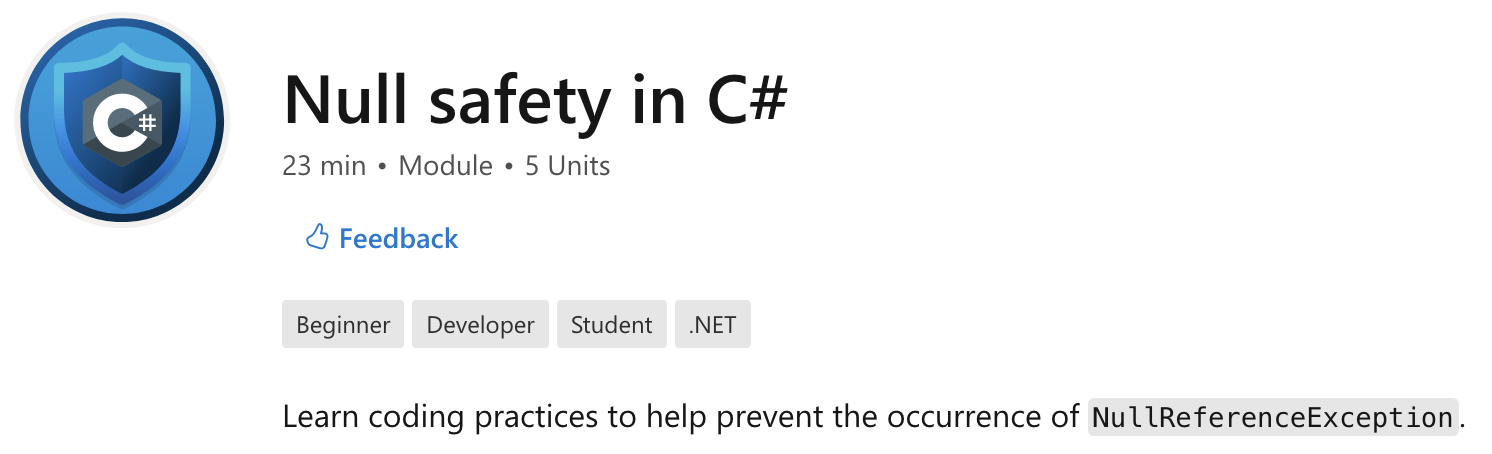
\includegraphics[width=0.65\textwidth]{csharp_null_safety.png}}}\pause

    \begin{alertblock}{Opinion}
        Constructors are a bad feature and very annoying to get right. They are detrimental to safety (constructors exists in a transient state) and to programmers.\note[itemize]{
            \item CROWD: do you actually know the exact order of initialization in constructors?
            \item Java has this weird thing where you call the super constructor as a normal code line but it has to be the first line in the constructor. Though they are relaxing it now a bit.
            \item Swift seems to be a language that invests most in safety of constructors
            \item We will come back to this but first we need to discuss type safety
        }
    \end{alertblock}
\end{frame}


\section{Type safety}


\begin{frame}[standout]
    \centering\large
    Make illegal states \textbf{unrepresentable}
\end{frame}

\begin{frame}
    \frametitle{Type safety}
    Here, a way to get rid of logic errors by usage of types. Illegal states are made impossible at compile time.

    Example: we want a type representing a list that is never empty.
    \begin{enumerate}
        \item encapsulating (meh)
        \item structural (good)
        \item formal (best)
    \end{enumerate}
\end{frame}

\subsection{NonEmptyList}

\begin{frame}[fragile]
    \frametitle{NonEmptyList}
    \framesubtitle{encapsulating}
    \begin{lstlisting}[language=Oop,gobble=8,basicstyle=\tt\scriptsize]
        class List<T> {
            func pop() -> T?
            func head() -> T?
            # other methods...
        }

        class NonEmptyList<T> extends List<T> {
            var data: List<T>

            constructor(data: List<T>) {
                if data.isEmpty { throw ArgumentError }
                self.data = data
            }

            override func pop() -> T { # return type is covariant
                if data.length == 1 { throw StateError }
                return data.pop()!
            }

            override func head() -> T { # return type is covariant
                return data.head()!
            }
        }
    \end{lstlisting}
\end{frame}

\begin{frame}
    \begin{itemize}
        \item Not really a subtype of \texttt{List}, cannot be used in its place
              \\$\to$ exceptions are not part of the signature
        \item Invariant-safe but not type-safe
        \item Are you sure all methods enforce the invariant?
    \end{itemize}
    \begin{alertblock}{Opinion}
        Exceptions are bad at modelling errors. \note[itemize]{
            \item expensive to implement
            \item require reasoning across functions (non local)
            \item fundamental thus hard to use when integrating with other languages
        } Unchecked exceptions are even worse. \note[itemize]{
            \item its not part of the API, makes internal changes possibly breaking changes
            \item zero clue what can actually go wrong
        }
    \end{alertblock}
\end{frame}

\subsection{Effect systems}

\begin{frame}{Effect systems}{Modeling side-effects}
    An \textbf{effect systems} concerns itself with modeling side effects of computations (printing to a console, reading a file, throwing exceptions, mutating global variables etc.). \note[itemize]{
        \item As seen in the previous example hiding those effects can lead to errors
    }

    Example effect systems:

    \begin{itemize}
        \item Java's checked exceptions
        \item Haskell's Monads
        \item OCaml's effect handlers
    \end{itemize}
\end{frame}

\begin{frame}{Algebraic effect handlers}
    Very powerful tool allowing a language to maintain purity while easily modeling all sorts of side effects. They also give us access to non-local control-flow.

    Using effect handlers we can implement without any help from the language such fundamental concepts as:

    \begin{itemize}
        \item (resumable) Exceptions
        \item Async/await
        \item break/continue in loops
    \end{itemize}
    \note[itemize]{
        \item All features listed above are very fundamental to languages that implement them. Effect handlers allow us to define these concepts on a library level.
    }

    \begin{alertblock}{Opinion}
        Using the \texttt{while (expr) {}} syntax is horrible. Why is the expr being evaluated many times with a different environment?
    \end{alertblock}
\end{frame}

\begin{frame}[fragile]{Implementing while}{Koka}
    \begin{lstlisting}[language=Koka,gobble=8,basicstyle=\tt\scriptsize]
        fun main()
          var p := 0
          while { True }
            p := p + 1
            if p == 11 then continue()
            if p > 10 then break()
          println(p)

        effect loop-flow
          ctl break() : a
          ctl continue() : a
        
        fun while(cond : () -> <div|e> bool,
                  block : () -> <div,loop-flow|e> ()) : <div|e> ()
          val do = handler
            ctl break() False
            ctl continue() True
            return(x) True
          
          if cond() then
            if do(block) then
              while(cond, block)
    \end{lstlisting}
    \note[itemize]{
        \item Koka is a research language from Microsoft Research
        \item It tries to make effect handlers ergonomic and efficient (effect handlers are usually expensive)
        \item Modeling code using algebraic effect handlers is a pure pleasure
        \item We strip the \texttt{wh} effect from the block
        \item We cannot call \texttt{brek} anywhere, there needs to be a handler
        \item You can even break from a different stack point
        \item \texttt{div} is an effect, unlike in Haskell
    }
\end{frame}

\begin{frame}[fragile]
    \frametitle{NonEmptyList}
    \framesubtitle{structural}
    Simple change: make the backing type unable to represent an empty list
    \begin{lstlisting}[language=Oop,gobble=8,basicstyle=\tt\scriptsize]
        class NonEmptyList<T> {
            var data: (T, List<T>)
            // ...
        }
    \end{lstlisting}
    We now have a guarantee that we cannot reach an illegal state
\end{frame}

\begin{frame}[fragile]
    \frametitle{NonEmptyList}
    \framesubtitle{formal}
    \begin{lstlisting}[language=lean,gobble=8,basicstyle=\tt\scriptsize]
        structure NonEmptyList (@$\alpha$@ : Type) where
            data : List @$\alpha$@
            notEmpty : !data.isEmpty
        
        def new (head : @$\alpha$@) (rest : List @$\alpha$@) : NonEmptyList @$\alpha$@ :=
          NonEmptyList.mk (head :: rest) (by
            unfold List.isEmpty
            split
            case _ => contradiction
            case _ => rfl
          )
        
        def head (l : NonEmptyList @$\alpha$@) : @$\alpha$@ :=
          l.data.head (by
            have h := l.notEmpty
            unfold List.isEmpty at h
            split at h
            case _ => contradiction
            case _ hq =>
              rewrite [hq]
              intro p
              contradiction
          )
    \end{lstlisting}
    \note[item]{Give a formal guarantee at each point in code that the list is not empty}
\end{frame}

\begin{frame}[fragile]
    \frametitle{Type promotion as formal proofs}
    \begin{lstlisting}[language=typescript,gobble=8,basicstyle=\tt\scriptsize]
        type NumOrStr = number | string

        function access(item: NumOrStr) {
            if (typeof item == "string") {
                item satisfies string
            } else {
                item satisfies number
            }
        }
    \end{lstlisting}
    \hrule
    \begin{lstlisting}[language=lean,gobble=8,basicstyle=\tt\scriptsize]
        inductive NumOrStr where | number | string
        
        def access (item : NumOrStr) :=
          if h : item = number then
            have _ : item = number := h
            ()
          else
            have _ : item = string := by
              cases item
              · contradiction
              · rfl
            ()
    \end{lstlisting}

    \note[item]{Passing proofs is a generalization of type promotion}
\end{frame}

\section{Runtime safety}

\begin{frame}[standout]
    \centering\large
    Not everything can be \textbf{guaranteed} at compile time
\end{frame}

\begin{frame}{Runtime safety}
    Things that are too hard to guarantee at compile time are done at runtime to maintain safety properties.

    Examples:

    \begin{itemize}
        \item Array bounds checks
        \item Null dereferencing
        \item Logic errors \note[item]{For example overlapping memory regions when doing a \texttt{memcpy}}
    \end{itemize}
\end{frame}

\begin{frame}{More important than static safety}
    We call a language memory safe if its runtime is safe.\note[item]{
        \item All garbage collected languages for example
        \item Bjarne got offended that C++ was deemed unsafe by the NSA. "No such language as C/C++"
    }

    \centering{
\includegraphics[width=\textwidth]{cpp_safety.jpg}}
\end{frame}

\begin{frame}[fragile]{Contemporary C++}
    \begin{columns}
        \begin{column}{0.5\textwidth}
            \begin{lstlisting}[gobble=16,language=Cpp,basicstyle=\tt\scriptsize]
                #include <iostream>
                
                int main() {
                  int a = 123;
                  int& b = a;
                
                  {
                    int newScope = 321;
                    b = newScope;
                  }
                
                  std::cout << b << std::endl;
                }
            \end{lstlisting}
        \end{column}
        \begin{column}{0.5\textwidth}
            \only<1>{\begin{checklist}
                    \item Exception is thrown?
                    \item Program crashes?
                    \item \texttt{b} is filled with garbage?
                    \item Your disk gets wiped
                \end{checklist}}
            \pause
            \only<2>{\begin{checklist}
                    \item[\done] Exception is thrown?
                    \item[\done] Program crashes?
                    \item[\done] \texttt{b} is filled with garbage?
                    \item[\done] Your disk gets wiped
                \end{checklist}}
        \end{column}
    \end{columns}
\end{frame}

\section{Typestate}

\begin{frame}[standout]
    \centering\large
    Don't read a file before opening it\note[itemize]{
        \item Enforcing logic invariants across function calls
        \item CROWD: Sounds simple, but how to enforce it?
    }
\end{frame}

\begin{frame}[fragile]{Typestate}
    \framesubtitle{What could possibly go wrong?}
    \begin{columns}
        \begin{column}{0.5\textwidth}
            \begin{lstlisting}[gobble=12,language=Cpp]
            #include <fstream>
    
            int main() {
              int num = 0;
              std::ifstream file;
            
              file >> num;
            
              file.close();
            }
            \end{lstlisting}
        \end{column}
        \begin{column}{0.5\textwidth}
            \only<1>{\begin{checklist}
                    \item Exception is thrown?
                    \item Program crashes?
                    \item \texttt{num} is filled with garbage?
                \end{checklist}}
            \pause
            \only<2>{\begin{checklist}
                    \item[\wontfix] Exception is thrown?
                    \item[\wontfix] Program crashes?
                    \item[\wontfix] \texttt{num} is filled with garbage?
                \end{checklist}}
            \note[itemize]{
                \item Nothing will happen, the error is hidden
                \item \texttt{file >> num} will return false
                \item It would be cool if a type system was able to protect us from such invariants (read can be done only if an open was done)
            }
        \end{column}
    \end{columns}
\end{frame}

\begin{frame}[fragile]{Augmenting types}
    \begin{columns}
        \begin{column}{0.5\textwidth}
            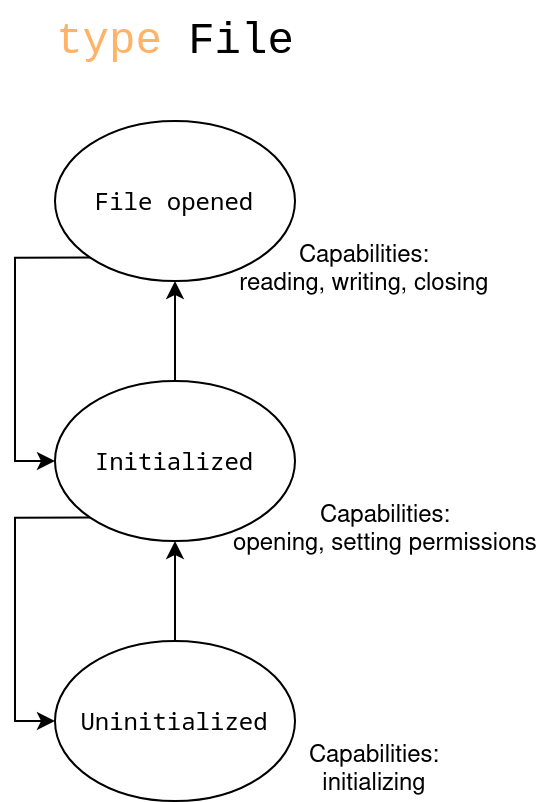
\includegraphics[height=0.8\textheight]{typestate.png}
        \end{column}
        \begin{column}{0.5\textwidth}
            \begin{lstlisting}[language=TypeState,gobble=16,basicstyle=\tt\tiny]
                typestate FileState =
                    uninitialized | initialized | opened

                class File with FileState {
                    func initialize()
                        when uninitialized
                        transition_to initialized
                    
                    func set_permission(flags: int)
                        when initialized
                    
                    func open(path: string)
                        when initialized
                        transition_to opened
                    
                    func read()
                        when opened -> string
                    
                    func write(data: string)
                        when opened
                    
                    func close()
                        when opened
                        transition_to initialized
                    
                    func deinitialize()
                        when initialized
                        transition_to uninitialized
                }
            \end{lstlisting}
        \end{column}
    \end{columns}
    \note[itemize]{
        \item Hard to do when aliasing exists. Aliasing is the bane of all cool feature.
        \item I don't know of any language which has them. No one is able to make them ergonomic enough.
    }
\end{frame}

\begin{frame}[fragile]{Late initialization}
    \framesubtitle{Typestates are already utilized!}
    \begin{lstlisting}[language=Dart,gobble=8,basicstyle=\tt\scriptsize]
        int a; // hidden typestate: uninitialized
        
        if (condition) {
            a = 123;
            // promoted to typestate initialized in this branch
        } else {
            // no promotion
        }
        // we take the infimum of both branches: typestate uninitialized
        
        print(a); // reading is not defined for typestate uninitialized!
    \end{lstlisting}\note[item]{Constructors kinda exist like in a typestate}
\end{frame}

\begin{frame}[fragile]{Simulating typestate in types}
    \begin{lstlisting}[language=Rust,gobble=8]
        enum FileState {
            Uninitialized, Initialized, Opened
        }

        struct File<S: FileState> {}

        impl<S: FileState> File<S> {
            fn new() -> File<Uninitialized>;
        }

        impl File<Opened> {
            fn read(&self) -> String;
        }

        impl File<Initialized> {
            fn open(self) -> File<Opened>;
        }
        // etc
    \end{lstlisting}
    \note[itemize]{
        \item In Rust its ok-ish because we can implement methods for specific types rather than whole classes
        \item Ownership in rust also helps (when changing state we consume ownership)
        \item Annoying in languages where we cannot shadow, as we will be often reassigning
        \item Not usable if this variable has to be shared
        \item Takeaway: use this pattern only when possible, File is a good candidate
    }
\end{frame}

\section{Proof assistants}

\begin{frame}[standout]
    \centering\large
    Pen and paper proofs are like languages without static types
\end{frame}

\begin{frame}{Proof assistants}
    \begin{itemize}
        \item Give guarantees about correctness
        \item Deep foundation in logic and computer science\note[item]{Watch out when talking to a logician, very easy to say something imprecise}
        \item Help humans write proofs
        \item Automate proof steps
        \item Currently meant to formalize not to discover
    \end{itemize}
\end{frame}

\begin{frame}{Usage in mathematics}
    \begin{itemize}
        \item First breakthrough is proving the \textit{four color theorem}
              \begin{center} 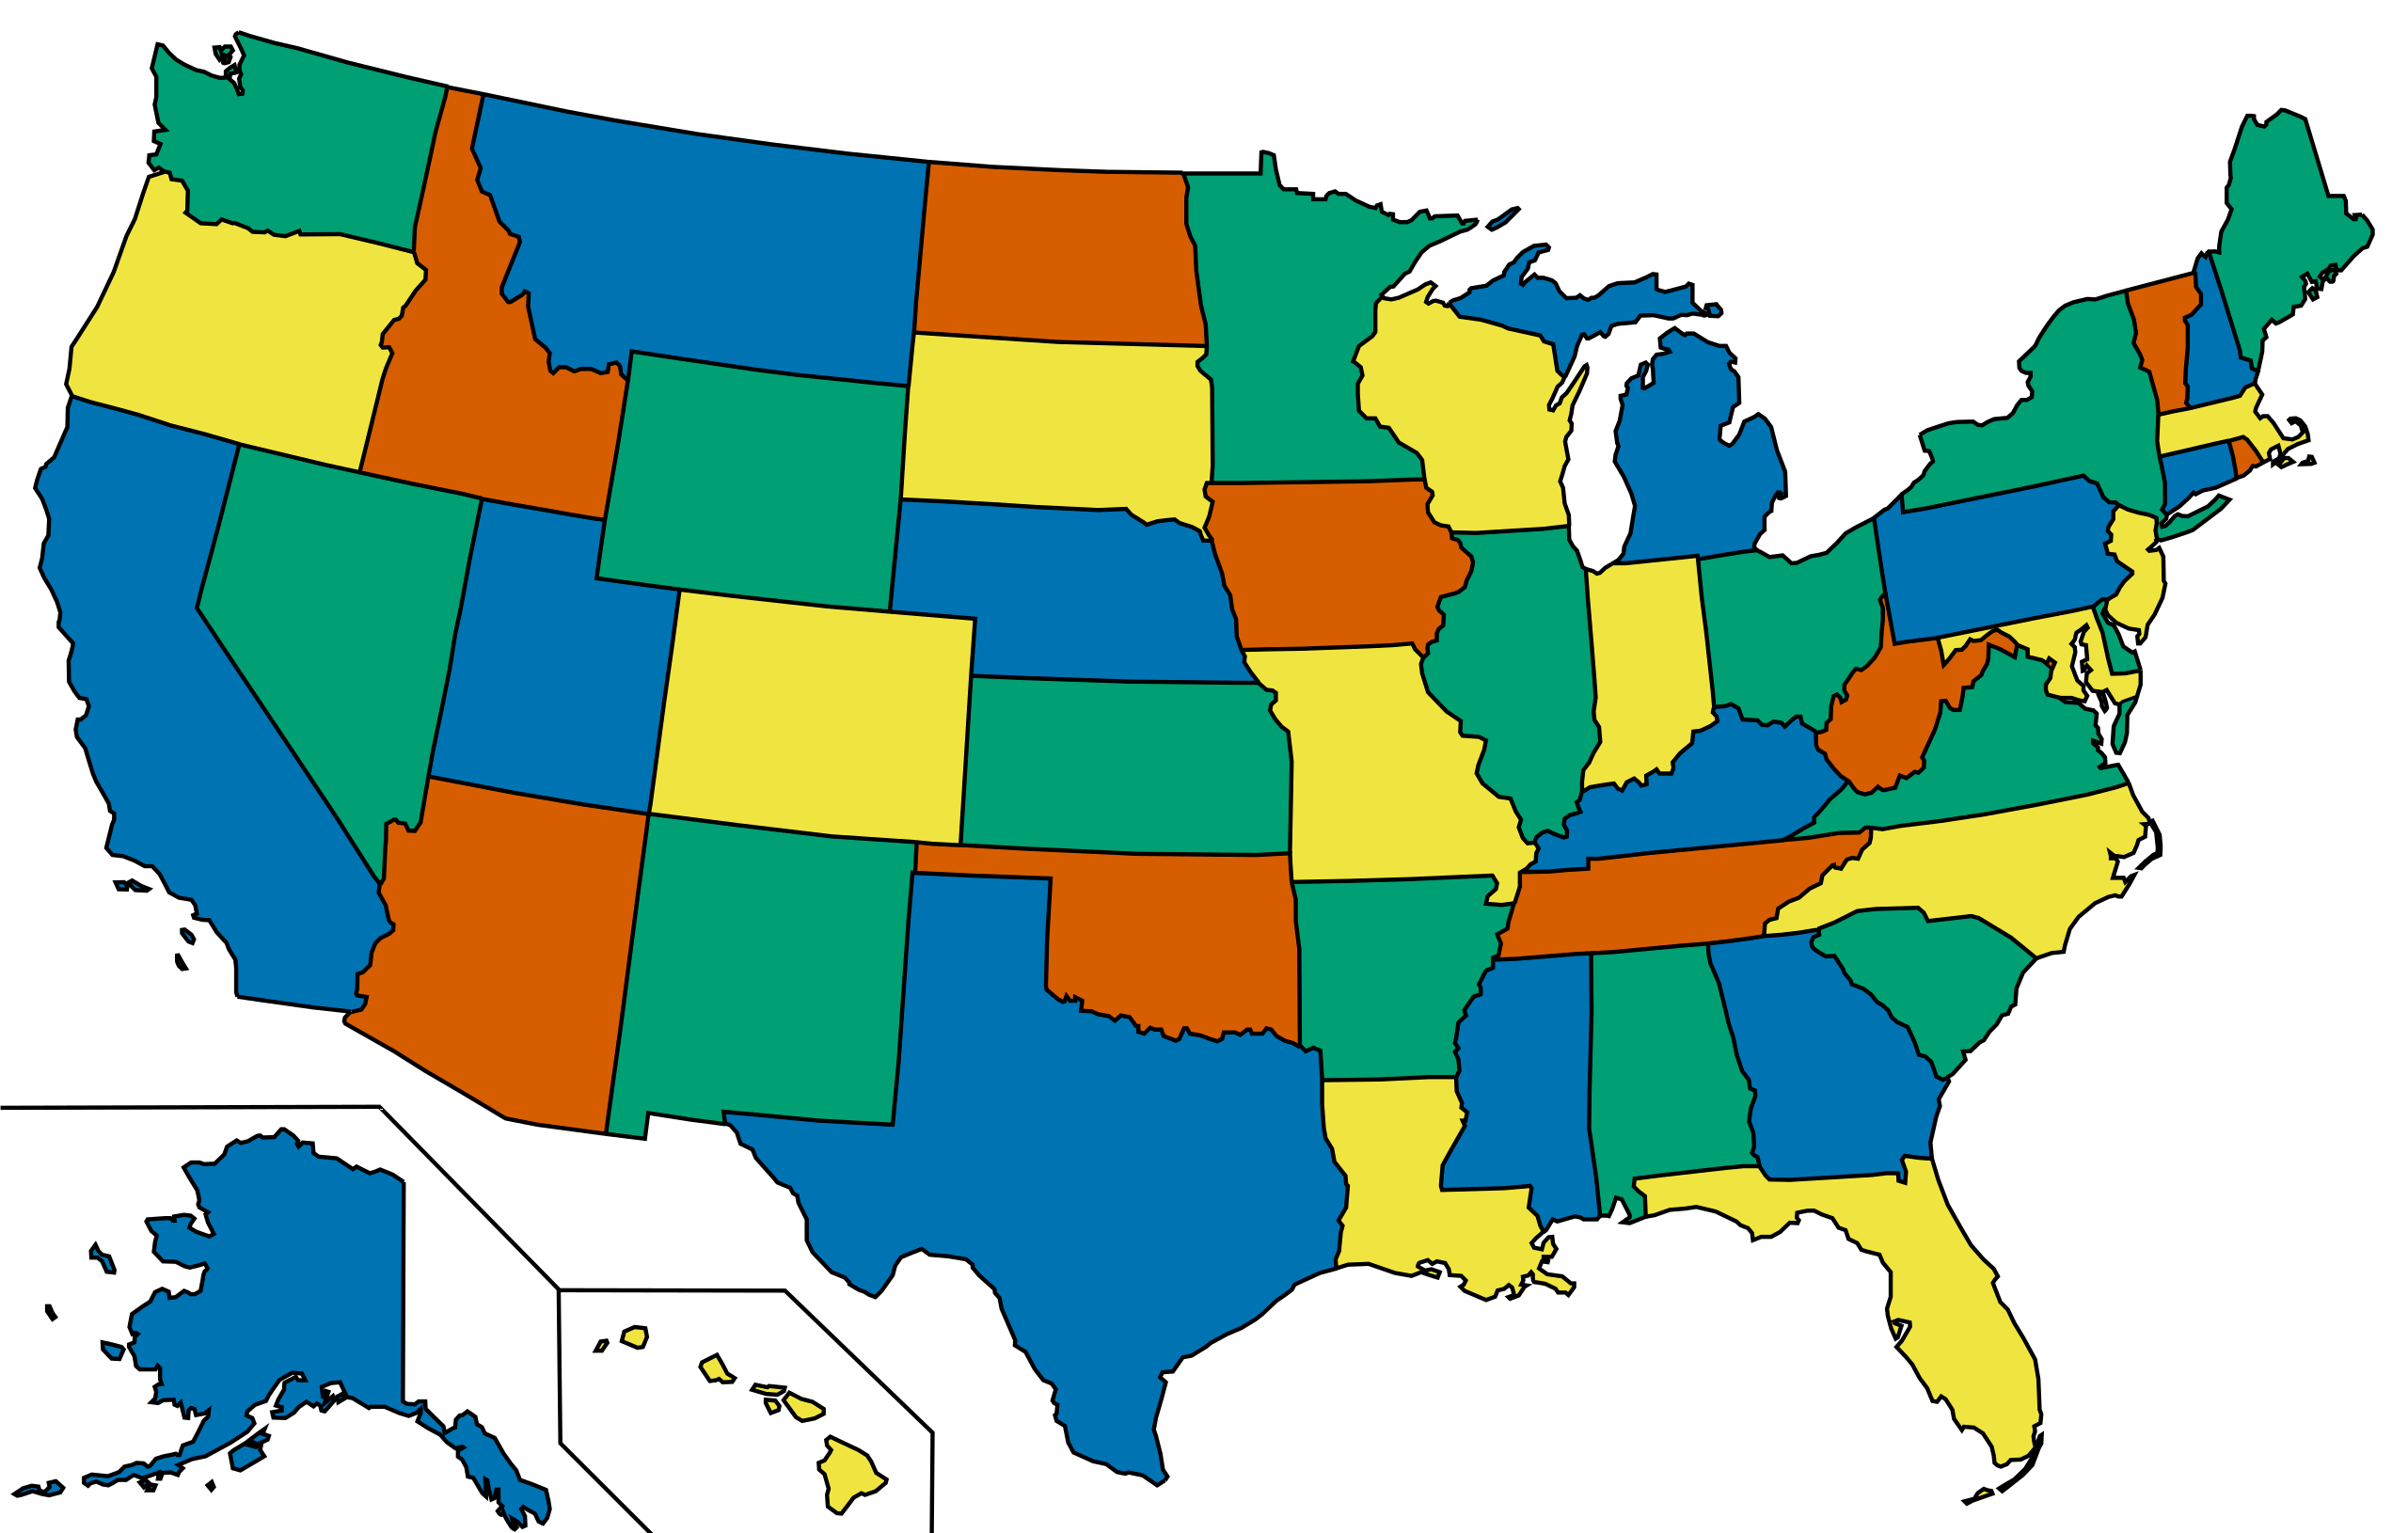
\includegraphics[width=0.3\textwidth]{map_coloring.png} \end{center}
        \item Recently some mathematicians picked up proof assistants
        \item Kevin Buzzard teaches using proof assistants at Imperial College
        \item Terrence Tao uses it to formalize his papers \\
              $\to$ recently he found a mistake in his paper!
    \end{itemize}
\end{frame}

\begin{frame}[fragile]{Example proof}
    \begin{theorem}
        The product of two even numbers is even.
    \end{theorem}

    \begin{proof}
        Let $a$, $b$ be two even numbers. So there exist $r$, $s$ such that $a = 2r$ and $b = 2s$. Therefore
        \begin{align}
            a \cdot b & = (2r)(2s)                  \\
                      & = 2 \cdot 2 \cdot r \cdot s \\
                      & = 4rs
        \end{align}
        So $a \cdot b$ is even because $\frac{4rs}{2} = 2rs$ which is a whole number.
    \end{proof}\note[itemize]{
        \item So many assumptions. CROWD: do you see any assumption?
        \item We need a "type system" to verify our proofs are correct
    }
\end{frame}

\begin{frame}{Programs are proofs}
    Turns out you can use programs as proofs (Curry–Howard correspondence). And you can reason about program using proofs. So you can reason about programs using programs.

    Proofs are nothing more than a program that is type checked.
\end{frame}

\begin{frame}
    \centering{\textit{(Demo)}}
\end{frame}

\begin{frame}{Drawbacks}
    \begin{itemize}
        \item Very fragile to underlying definitions and implementations
        \item Very time consuming to write proofs \\
              $\to$ especially when you waste time trying to prove something false
        \item Human factor is still at play: someone has to state the properties \\
              $\to$ leads to "bugs", we proved not what we meant
        \item Proofs are not very readable
    \end{itemize}
\end{frame}


\End
\begin{frame}[plain, standout]
    \centering
    Current software \textit{sucks}, \\we \textit{know} how to do better, \\but it is \textit{expensive}.
    \vfill
    Only AI can save us.
\end{frame}

\begin{frame}[plain]
    \centering
    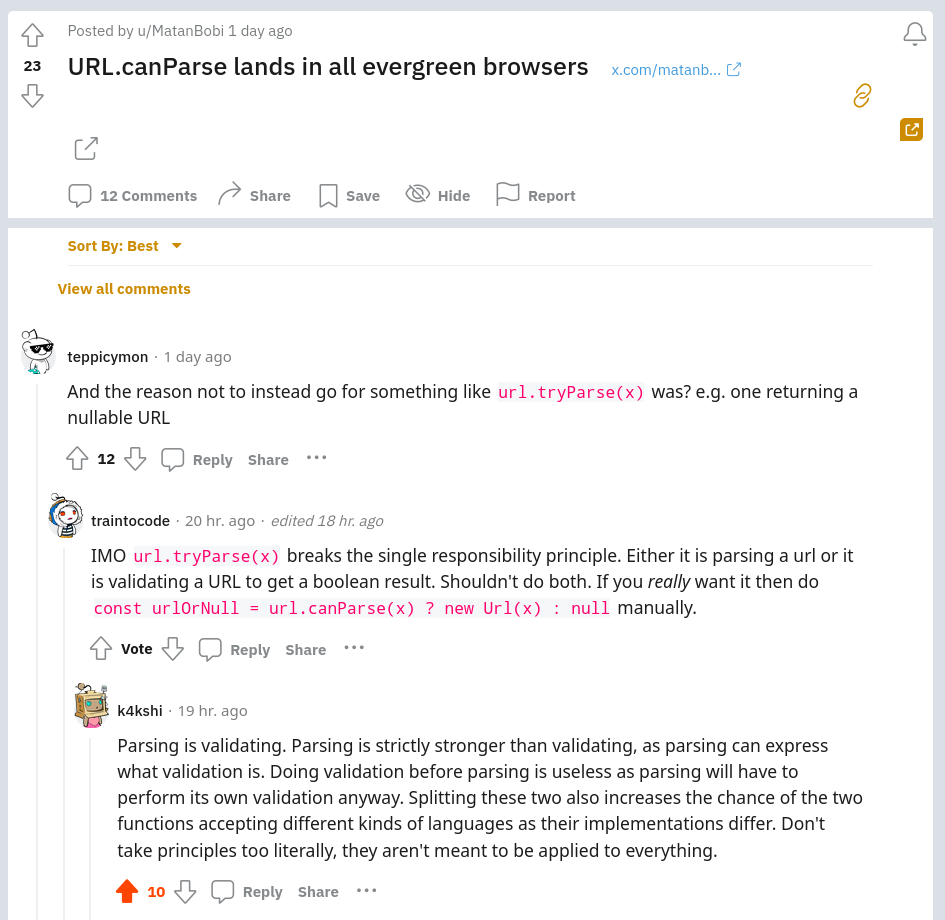
\includegraphics[height=\textheight]{url_can_parse.png}
\end{frame}

\end{document}
